{
    \begin{figure*}[ht!]
        \centering
        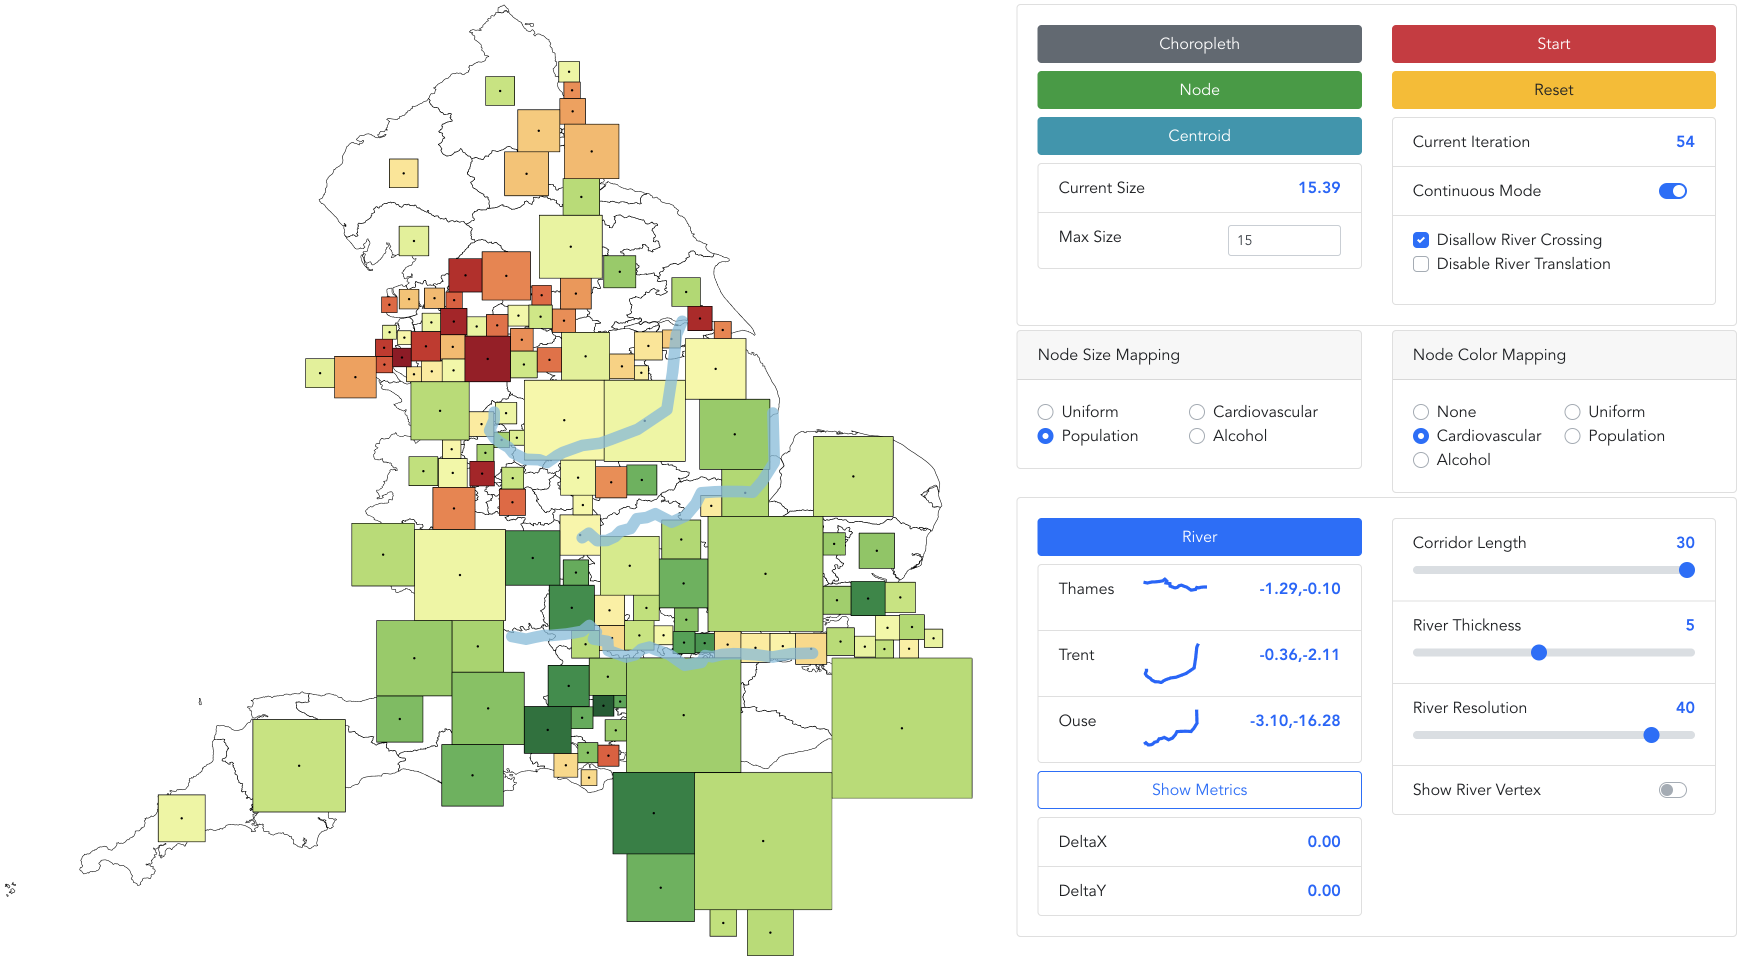
\includegraphics[width=0.8\textwidth,keepaspectratio]{figure/UI.png}
        \caption{A screenshot of the software. User options are provided to adjust the size, color mapping, visibility of nodes and rivers. Other options include the ability to control the overlap removal behavior: rivers can be static, dynamic, or constrained [why too complicated? this is what we are doing in the software].}
        \label{fig:overview}
    \end{figure*}
}

\section{Introduction and Motivation}

Cartograms are representations of hybrid geographical and abstract data based on a value-by-area mapping combining statistical and geographical information \cite{dent2009Cartography}. Various styles of cartograms have been proposed and implemented, covering applications such as urban planning \cite{harris2018Mapping, arranz-lopez2021Enduser}, natural hazard forecasting \cite{pappenberger2019Cartograms, park2020Flood}, conservation and environmental planning \cite{galluzzi2018Mapping, rocchini2019Cartogramming}, political and social demographics \cite{breitzman2018Using, alieva2021How}, and public health decision-making \cite{gao2020Visualising, sack2021Visualizing}.

Among the four types of cartograms categorized by \citea{nusrat2016State} (contiguous, non-contiguous, rectangular, and Dorling), a trade-off between types of accuracy is made (See \Cref{table:accuracy}). For this project, we focus on non-contiguous cartograms like Demers cartograms, because they facilitate statistical comparison between regions and they can make good use of screen space. Building on Demers cartograms \cite{ian2002Cartogram}, we introduce and develop novel dynamic topological features, such as rivers, aiming to improve the readability and geographical accuracy without sacrificing statistical accuracy. Standard Demers cartograms are composed of uniform shape nodes. As such, this can reduce their legibility. We implement a new cartographic layout algorithm that includes rivers into the layout of the nodes representing geographical regions. Introducing rivers into the cartogram improves their legibility. To reduce geographical errors and make efficient use of screen space, the algorithm also updates the position of rivers to accommodate the node layout. We then apply the algorithm to a real-world case study using an Electronic Health Records (EHR) dataset to evaluate the result. We present a user study demonstrating its effectiveness.

Our contributions include:

\begin{itemize}
    \item A new variant of Demers cartograms that incorporates rivers to improve readability and recognizability,
    \item A novel layout algorithm that preserves node positions relative to dynamic topological features such as rivers,
    \item A user study evaluation of the technique with an application to EHRs.
\end{itemize}

The results of the user study indicate that rivers can improve the legibility of cartograms. One of the major challenges involved is how to develop a layout algorithm that handles different shapes. In other words, the layout algorithm is novel because it handles different types of nodes -- rectangular representing regions and polylines representing rivers. Another challenge we overcome in developing the algorithm is to resolve stalemate situations introduced by dynamic rivers while minimizing geographical error.